\section{Results}\label{sec:results}

%#TODO plot RMV and RMSE against each other like busk2021

%#TODO husk at kommentere på epistemisk usikkerhed, forbundet med grafer og metriker

%#TODO test_loss_128 mean: 36.799533534049985, testloss_64 mean: 37.081851065158844

%#TODO gennemsnitlig varians over ensemble i testsets for 64: 0.29809390719701073 og for 128: 0.15309279243460014

%#TODO ence for MPNN64 ensemble: 23.50 , 128: 32.06

%# ensemble vs. single models() first ensemble model); 64: [0.969972792480524, 0.9676276973022239, 0.9888736279961788, 0.9828243429827256, 0.9988442451349356, 1.2097879561835665], 128: [0.9900557188310352, 1.0342352502056764, 1.017243472314507, 1.0004067356869728, 1.0409579224317915, 1.0105280059508281]

%#TODO sammenlign MSE for ensemble64: 0.96 og ensemble128: 0.99

%#TODO nævn noget med at training loss og val loss data kun gemmes med lav frekvens, derfor er der sammenfald på mange af batch længderne
%#TODO nævn noget med at early stopping blev triggered, men ikke stoppede før den fulde epoch var færdig. derfor kommer både loss og number of gradient steps i intervaller af 315


\begin{table}[H]
    \centering
    \caption{Number of gradient steps, for individual models in ensembles}
    \label{tab:num-steps}
    \begin{tabular}{|cccc|}
    \hline
    \multicolumn{4}{|c|}{\textbf{MPNN ensembles total gradient steps}}                                                                         \\ \hline
    \multicolumn{2}{|c|}{\textit{\textbf{MPNN128 Ensemble}}}                        & \multicolumn{2}{c|}{\textit{\textbf{MPNN64 Ensemble}}}   \\ \hline
    \multicolumn{1}{|c|}{\textbf{Model}}      & \multicolumn{1}{c|}{\textit{Value}} & \multicolumn{1}{c|}{\textbf{Model}}     & \textit{Value} \\ \hline
    \multicolumn{1}{|c|}{\textbf{MPNN128\_1}} & \multicolumn{1}{c|}{630}            & \multicolumn{1}{c|}{\textbf{MPNN64\_1}} & 630            \\ \hline
    \multicolumn{1}{|c|}{\textbf{MPNN128\_2}} & \multicolumn{1}{c|}{630}            & \multicolumn{1}{c|}{\textbf{MPNN64\_2}} & 945            \\ \hline
    \multicolumn{1}{|c|}{\textbf{MPNN128\_3}} & \multicolumn{1}{c|}{630}            & \multicolumn{1}{c|}{\textbf{MPNN64\_3}} & 630            \\ \hline
    \multicolumn{1}{|c|}{\textbf{MPNN128\_4}} & \multicolumn{1}{c|}{630}            & \multicolumn{1}{c|}{\textbf{MPNN64\_4}} & 945            \\ \hline
    \multicolumn{1}{|c|}{\textbf{MPNN128\_5}} & \multicolumn{1}{c|}{945}            & \multicolumn{1}{c|}{\textbf{MPNN64\_5}} & 630            \\ \hline
    \end{tabular}
    \end{table}

    \begin{table}[H]
        \centering
        \caption{Training time for individual models in ensembles, and total training time.}
        \label{tab:train-time}
        \begin{tabular}{|cccccl|}
        \hline
        \multicolumn{6}{|c|}{\textbf{MPNN Total Training Time}}                                                                                                                                                                                                            \\ \hline
        \multicolumn{3}{|c|}{\textit{\textbf{MPNN128 Ensemble}}}                                                                         & \multicolumn{3}{c|}{\textit{\textbf{MPNN64 Ensemble}}}                                                                          \\ \hline
        \multicolumn{1}{|c|}{\textbf{Model}}                  & \multicolumn{1}{c|}{\textit{Value}} & \multicolumn{1}{c|}{\textit{Unit}} & \multicolumn{1}{c|}{\textbf{Model}}                  & \multicolumn{1}{c|}{\textit{Value}} & \multicolumn{1}{c|}{\textit{Unit}} \\ \hline
        \multicolumn{1}{|c|}{\textbf{MPNN128\_1}}             & \multicolumn{1}{c|}{383}            & \multicolumn{1}{c|}{minutes}       & \multicolumn{1}{c|}{\textbf{MPNN64\_1}}              & \multicolumn{1}{c|}{368}            & minutes                            \\ \hline
        \multicolumn{1}{|c|}{\textbf{MPNN128\_2}}             & \multicolumn{1}{c|}{473}            & \multicolumn{1}{c|}{minutes}       & \multicolumn{1}{c|}{\textbf{MPNN64\_2}}              & \multicolumn{1}{c|}{551}            & minutes                            \\ \hline
        \multicolumn{1}{|c|}{\textbf{MPNN128\_3}}             & \multicolumn{1}{c|}{384}            & \multicolumn{1}{c|}{minutes}       & \multicolumn{1}{c|}{\textbf{MPNN64\_3}}              & \multicolumn{1}{c|}{370}            & minutes                            \\ \hline
        \multicolumn{1}{|c|}{\textbf{MPNN128\_4}}             & \multicolumn{1}{c|}{455}            & \multicolumn{1}{c|}{minutes}       & \multicolumn{1}{c|}{\textbf{MPNN64\_4}}              & \multicolumn{1}{c|}{559}            & minutes                            \\ \hline
        \multicolumn{1}{|c|}{\textbf{MPNN128\_5}}             & \multicolumn{1}{c|}{668}            & \multicolumn{1}{c|}{minutes}       & \multicolumn{1}{c|}{\textbf{MPNN64\_5}}              & \multicolumn{1}{c|}{375}            & minutes                            \\ \hline
        \multicolumn{1}{|c|}{\textit{\textbf{Total minutes}}} & \multicolumn{1}{c|}{2363}           & \multicolumn{1}{c|}{minutes}       & \multicolumn{1}{c|}{\textit{\textbf{Total minutes}}} & \multicolumn{1}{c|}{2223}           & \multicolumn{1}{c|}{minutes}       \\ \hline
        \multicolumn{1}{|c|}{\textit{\textbf{Total hours}}}   & \multicolumn{1}{c|}{39.38}          & \multicolumn{1}{c|}{hours}         & \multicolumn{1}{c|}{\textit{\textbf{Total hours}}}   & \multicolumn{1}{c|}{37.1}           & \multicolumn{1}{c|}{hours}         \\ \hline
        \end{tabular}
        \end{table}


\begin{figure}[H]
    \caption{Plots of training loss for individual models in the ensembles of 64-state- and 128-state- representations.}
    \begin{subfigure}{0.5\textwidth}
        \centering
        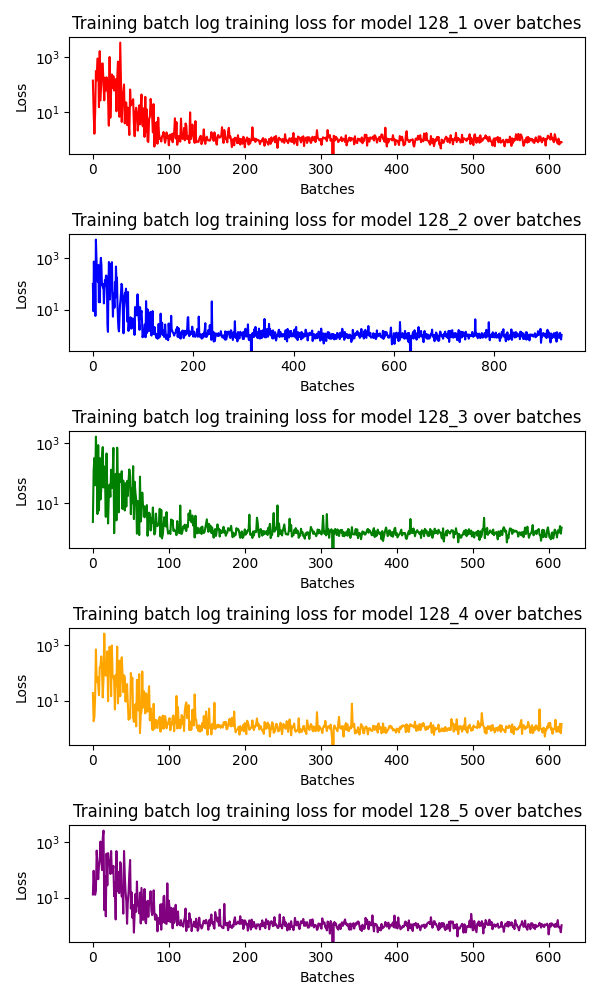
\includegraphics[width=0.95\linewidth]{Images/Results/Training_loss_128.png}
        \caption{1a}
        \label{fig:t-loss-128}
    \end{subfigure}%
    \begin{subfigure}{0.5\textwidth}
        \centering
        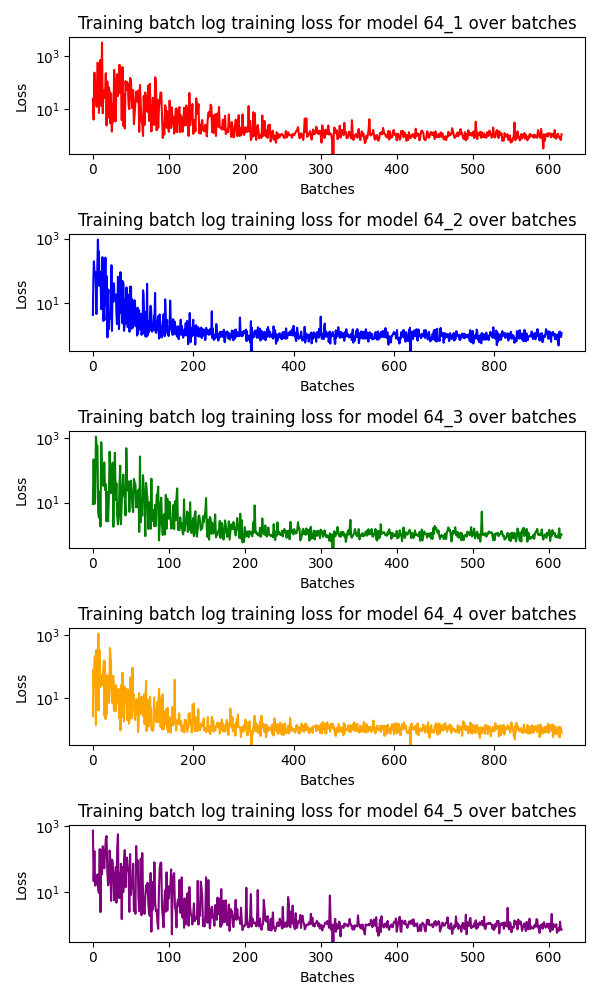
\includegraphics[width=0.95\linewidth]{Images/Results/Training_loss_64.png}
        \caption{1b}
        \label{fig:t-loss-64}
    \end{subfigure}
    \label{fig:t-loss}
\end{figure}

\begin{figure}[H]
    \caption{Plots of training loss for individual models in the ensembles of 64-state- and 128-state- representations.}
    \begin{subfigure}{0.5\textwidth}
        \centering
        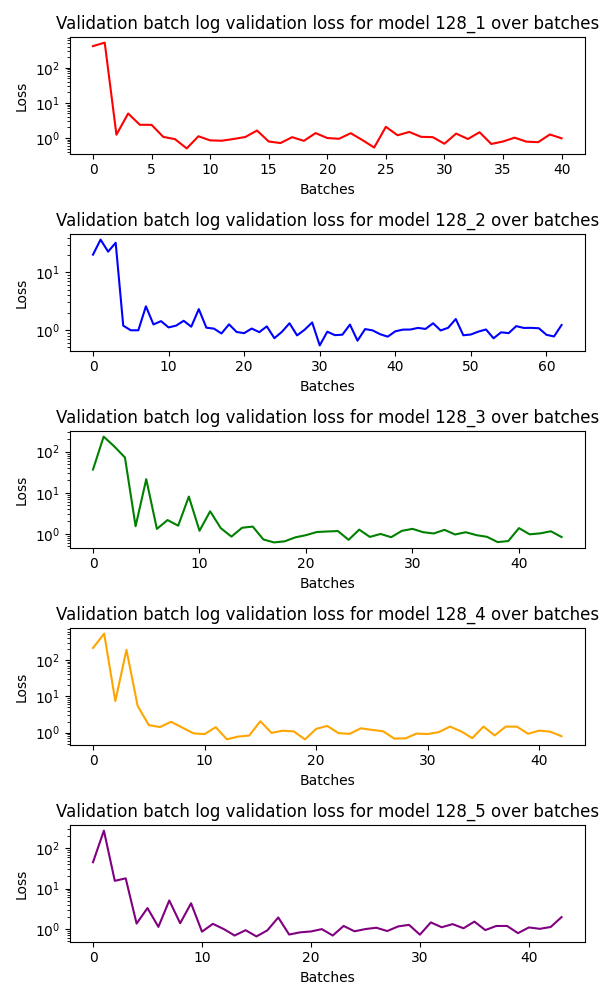
\includegraphics[width=0.95\linewidth]{Images/Results/Validation_loss_128.png}
        \caption{1a}
        \label{fig:v-loss-128}
    \end{subfigure}%
    \begin{subfigure}{0.5\textwidth}
        \centering
        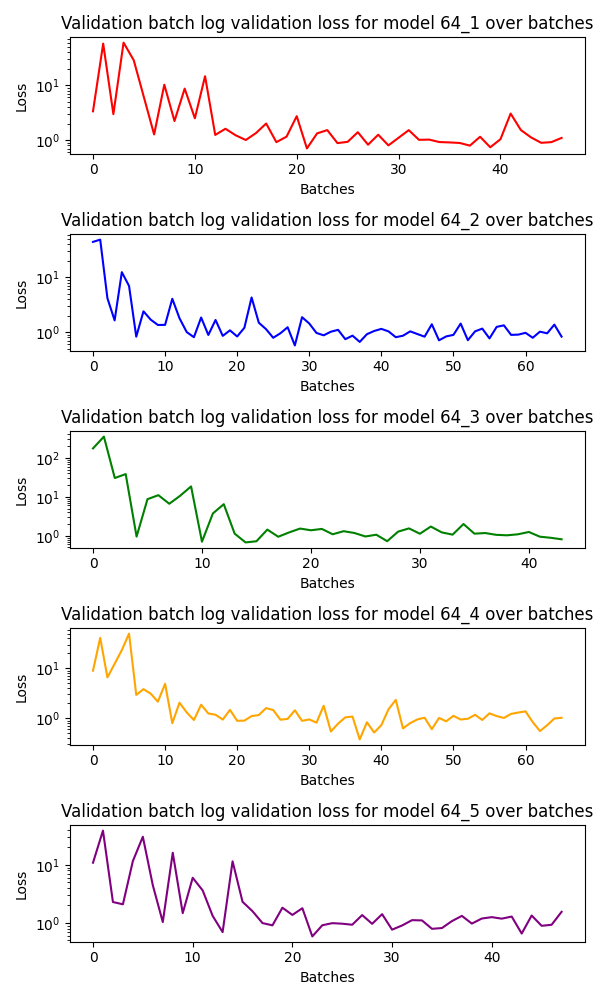
\includegraphics[width=0.95\linewidth]{Images/Results/Validation_loss_64.png}
        \caption{1b}
        \label{fig:v-loss-64}
    \end{subfigure}
    \label{fig:v-loss}
\end{figure}

\newpage


